\documentclass[a4paper]{article}
\usepackage[utf8]{inputenc}
\usepackage[T1]{fontenc}
\usepackage{url}
\usepackage{tikz}
\usepackage{csvsimple}

\title{2-24-1 Optimization and search heuristics}
\author{Baptiste Louf, Yann Ramusat}

\begin{document}
\maketitle

For the purpose of the project we have implemented most of the algorithms seen during the first part of the course.
In addition to the \textit{RLS} and \textit{(1+1)EA} that are already part of the bootstrap project we propose the \textit{($\mu$+$\lambda$)EA}, the \textit{($\mu$,$\lambda$)EA}, the \textit{simulated annealing} and the \textit{1+($\lambda$,$\lambda$)GA}.

We also use an heuristic to identify useless object and delete them. You can find more information for this processing in INSERT REF.

We will discuss about the impact of the preprocessing, the optimal parameters $\lambda$ and $\mu$ for each algorithm and we will compare the differents heuristics over different kind of instances.

TODO PRECISE CONFIG OF THE PC.

\tableofcontents

\newpage

\section{Preprocessing}

We begin with a comparison of the effectiveness of the \textit{RLS} with and without the preprocessing. This will give an insight of the utility of this method. We consider the dataset \textbf{fnl4461 n4460 bounded-strongly-corr 01}.

\begin{figure}[!h]
	\begin{center}
		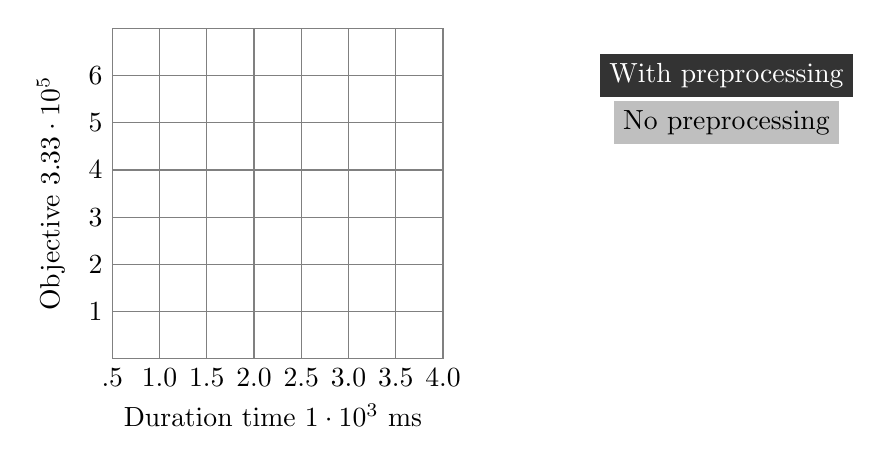
\begin{tikzpicture}[scale = 0.6]
			\draw[step=1,gray,thin]  (0,0) grid (7,7);
			\foreach \x in {.5,1.0,1.5,2.0,2.5,3.0,3.5,4.0}
		 \node[anchor=north] at (2*\x-1,0) {\x};
			\foreach \y in {1,2,3,4,5,6}
		 \node[anchor=east] at (0,\y) {\y};
			\draw (3.4,-1.2) node{Duration time $1\cdot10^3$ ms};
			\draw (-1.3,3.5) node[rotate=90]{Objective $3.33\cdot10^5$};
			
			\draw[thick] plot[mark=*]  file {with_preproc.txt};
			\draw[thick, color=gray] plot[mark=+] file {no_preproc.txt};
			
			\draw[white] (13,6)node[fill=black!80] {With preprocessing};
			\draw(13,5)node[fill=gray!50] {No preprocessing};
		\end{tikzpicture}
	\end{center}
	\caption{Effectiveness with and without preprocessing.}
	\label{expe_preprocessing}
\end{figure}

This suggests the preprocessing is not so usefull. In the following tests we will assume the preprocessing is desactivated.

\section{Finding optimal parameters}

We now search for optimal values for the parameters given to the \textit{Evolutionary Algorithms}.

\subsection{Parameters for the ($\mu$+$\lambda$)EA}

We have computed results over the same dataset as before but with a time limit fixed to $2$ seconds.

In the following table we give the objective value ($\cdot 10^3$) depending on $\lambda$ (columns) and $\mu$ (rows). 

\csvautotabular{mu+lambda.csv}

We do not represent greater values of $\mu$ because they are worth.

We observe that definitively, the best value for $\mu$ is $1$ and that $\lambda$ can be taken around $5$ or $6$.


\subsection{Parameters for the ($\mu$,$\lambda$)EA}

\section{Comparisons}

\end{document}